\documentclass[../../../main.tex]{subfiles}
\begin{document}

%%%%%%%%%%%%%%%%%%%%%%%%%%%%%%%%%%%%%%%%%
%%%%%%%%%%%%%%%%%%%%%%%%%%%%%%%%%%%%%%%%%
%%%%%%%%%%%%%%%%%%%%%%%%%%%%%%%%%%%%%%%%%
\chapter{The location of the data}

Earlier, we mentioned that a \vocab{statistic} is a sort of summary number. I call it a summary value because it summarizes a bunch of values in a certain way. By looking just at the summary number, you can get a particular viewpoint on the values, without having to look at all the observations yourself. Here we will talk about a particular family of statistics (i.e., summary numbers). These are called the \vocab{median}, \vocab{quartiles}, and \vocab{percentiles}.

The idea is pretty straight forward. Take a number of observations, and order them into a sequence that goes from the lowest to the highest value. Then divide that ordered sequence up into equal sized chunks. For example, you can cut the sequence into two halves, or into four quarters, or even into a hundred hundredths. Then look at the values at the cut points. Knowing the values of the cut points tells us what, say, the middle value of the sequence is. 


%%%%%%%%%%%%%%%%%%%%%%%%%%%%%%%%%%%%%%%%%
%%%%%%%%%%%%%%%%%%%%%%%%%%%%%%%%%%%%%%%%%
\section{The median}

The \vocab{median} of a data set is a value that cuts the values in the data set into two halves, so that the same number of values are in each half.


%%%%%%%%%%%%%%%%%%%%%%%%%%%%%%%%%%%%%%%%%
\subsection{How to compute it}

To compute the median, follow these steps.

\begin{itemize}
  \item Order the data from lowest to highest.
  \item Cut the ordered data set into two halves, so that each half has the same number of values in it.
  \item The median is at the cut point.
\end{itemize}


%%%%%%%%%%%%%%%%%%%%%%%%%%%%%%%%%%%%%%%%%
\subsection{Example 1} 

Suppose we have a data set with these values:

\begin{center}
  6 2 1 4 3 5
\end{center}

\noindent
First order them from lowest to highest:

\begin{center}
  \begin{tikzpicture}

    \node at (-4, -1) {1};
    \node at (-2, -1) {2};
    \node at (0, -1) {3};
    \node at (2, -1) {4};
    \node at (4, -1) {5};
    \node at (6, -1) {6};

  \end{tikzpicture}
\end{center}

\noindent
Draw a line that cuts the set in half:

\begin{center}
  \begin{tikzpicture}

    \node at (-4, -1) {1};
    \node at (-2, -1) {2};
    \node at (0, -1) {3};
    \node at (2, -1) {4};
    \node at (4, -1) {5};
    \node at (6, -1) {6};

    \draw[-] (1, 0) -- (1, -2);

  \end{tikzpicture}
\end{center}

\noindent
The median is precisely at that dividing line. In particular, it's the number that's exactly half way between the two middle numbers. In this case, the two middle numbers are 3 and 4, and 3.5 is exactly half way between them. So the median is 3.5:

\begin{center}
  \begin{tikzpicture}

    \node at (-4, -1) {1};
    \node at (-2, -1) {2};
    \node at (0, -1) {3};
    \node at (2, -1) {4};
    \node at (4, -1) {5};
    \node at (6, -1) {6};

    \draw[-] (1, 0) -- (1, -2);
    \draw[<-] (1, -2.25) -- (1, -2.75);
    \node at (1, -3) {Median (3.5)};

  \end{tikzpicture}
\end{center}

\noindent
Note that there are exactly the same number of values on the left side and the right side of the line:

\begin{center}
  \begin{tikzpicture}

    \node at (-4, -1) {1};
    \node at (-2, -1) {2};
    \node at (0, -1) {3};
    \node at (2, -1) {4};
    \node at (4, -1) {5};
    \node at (6, -1) {6};

    \draw[-] (-4.5, -1) -- (-4.5, -1.5) -- (0.5, -1.5) -- (0.5, -1);
    \draw[<-] (-2, -1.75) -- (-2, -2.25);
    \node at (-2, -2.5) {3 values};

    \draw[-] (1, 0) -- (1, -2);
    \draw[<-] (1, -2.25) -- (1, -2.75);
    \node at (1, -3) {Median (3.5)};

    \draw[-] (1.5, -1) -- (1.5, -1.5) -- (6.5, -1.5) -- (6.5, -1);
    \draw[<-] (4, -1.75) -- (4, -2.25);
    \node at (4, -2.5) {3 values};

  \end{tikzpicture}
\end{center}


%%%%%%%%%%%%%%%%%%%%%%%%%%%%%%%%%%%%%%%%%
\subsection{Example 2} 

Suppose we have this data set:

\begin{center}
  1 2.2 2.2 3.6 3.8 7
\end{center}

\noindent
What's the median? It's the number that's exactly half way between the middle two values. In this case, the two middle numbers are 2.2 and 3.6. Half way between them is 2.8:

\begin{center}
  \begin{tikzpicture}

    \node at (-4, -1) {1};
    \node at (-2, -1) {2.2};
    \node at (0, -1) {2.2};
    \node at (2, -1) {3.6};
    \node at (4, -1) {3.8};
    \node at (6, -1) {7};

    \draw[-] (1, 0) -- (1, -2);
    \draw[<-] (1, -2.25) -- (1, -2.75);
    \node at (1, -3) {Median (2.8)};

  \end{tikzpicture}
\end{center}


%%%%%%%%%%%%%%%%%%%%%%%%%%%%%%%%%%%%%%%%%
\subsection{Example 3} 

What if there are an odd number of values? Take this data set:

\begin{center}
  1 2 2 8 10
\end{center}

\noindent
We still draw a line exactly in the middle, to cut the data set into two halves:

\begin{center}
  \begin{tikzpicture}

    \node at (-4, -1) {1};
    \node at (-2, -1) {2};
    \node at (0, -1) {2};
    \node at (2, -1) {8};
    \node at (4, -1) {10};

    \draw[-] (0, 0) -- (0, -2);
    \draw[<-] (0, -2.25) -- (0, -2.75);
    \node at (0, -3) {Median (2)};

  \end{tikzpicture}
\end{center}

\noindent
Now the line cuts right through a number. But that's okay. It still cuts the data set into two equally sized halves. There are the same number of elements on both sides of the cut line. If you don't include the middle number in either half, there are 2 values on each side:

\begin{center}
  \begin{tikzpicture}

    \node at (-4, -1) {1};
    \node at (-2, -1) {2};
    \node at (0, -1) {2};
    \node at (2, -1) {8};
    \node at (4, -1) {10};

    \draw[-] (-4.5, -1) -- (-4.5, -1.5) -- (-1.5, -1.5) -- (-1.5, -1);
    \draw[<-] (-3, -1.75) -- (-3, -2.25);
    \node at (-3, -2.5) {2 values};

    \draw[-] (0, 0) -- (0, -2);
    \draw[<-] (0, -2.25) -- (0, -2.75);
    \node at (0, -3) {Median (2)};

    \draw[-] (1.5, -1) -- (1.5, -1.5) -- (4.5, -1.5) -- (4.5, -1);
    \draw[<-] (3, -1.75) -- (3, -2.25);
    \node at (3, -2.5) {2 values};

  \end{tikzpicture}
\end{center}

\noindent
If you do include the middle number in each half, you still get the same number of values on each side:

\begin{center}
  \begin{tikzpicture}

    \node at (-4, -1) {1};
    \node at (-2, -1) {2};
    \node at (0, -1) {2};
    \node at (2, -1) {8};
    \node at (4, -1) {10};

    \draw[-] (-4.5, -1) -- (-4.5, -1.5) -- (0.5, -1.5) -- (0.5, -1);
    \draw[<-] (-2, -1.75) -- (-2, -2.25);
    \node at (-2, -2.5) {3 values};

    \draw[-] (0, 0) -- (0, -2);
    \draw[<-] (0, -2.25) -- (0, -2.75);
    \node at (0, -3) {Median (2)};

    \draw[-] (-0.5, -1) -- (-0.5, -1.5) -- (4.5, -1.5) -- (4.5, -1);
    \draw[<-] (2, -1.75) -- (2, -2.25);
    \node at (2, -2.5) {3 values};

  \end{tikzpicture}
\end{center}


%%%%%%%%%%%%%%%%%%%%%%%%%%%%%%%%%%%%%%%%%
\subsection{Calculate the midway point} 

To find the number that is exactly half way between the two middle values $v_{1}$ and $v_{2}$, add the two values together, and divide the result by 2:

\begin{equation*}
  \frac{v_{1} + v_{2}}{2}
\end{equation*}

\noindent
For example:

\begin{itemize}

  \item 
    Half way between 2 and 4:
    \begin{equation*}
      \frac{2 + 4}{2} = \frac{6}{2} = 3
    \end{equation*}
    
  \item 
    Half way between 2 and 2:
    \begin{equation*}
      \frac{2 + 2}{2} = \frac{4}{2} = 2
    \end{equation*} 
    
   \item 
    Half way between 2.2 and 3.4:
    \begin{equation*}
      \frac{2.2 + 3.4}{2} = \frac{5.6}{2} = 2.8
    \end{equation*} 

\end{itemize}


%%%%%%%%%%%%%%%%%%%%%%%%%%%%%%%%%%%%%%%%%
\subsection{Interpreting the median}

What does the median tell us? It tells us that at least half of the values in the data set have a value less than or equal to it. Because the values are ordered, you can go to the median, and you know that the values below it are going to be equal to or less than it. Look at the examples from above:

\begin{itemize}
  \item In example 1, half of the values are less than or equal to 3.5. Look at the example, and count how many values are less than 3.5. Indeed, there are 3 values that are less than or equal to 3.5, out of a total of 6 values in the data set.
  
  \item In example 2, half of the values are less than or equal to 2.8. Confirm this by looking at the example. There are 3 values (out of a total of 6) that are less than or equal to 2.8.
  
  \item In example 3, half of the values are again less than or equal to 2. You can confirm this by looking at the example.

\end{itemize}


%%%%%%%%%%%%%%%%%%%%%%%%%%%%%%%%%%%%%%%%%
%%%%%%%%%%%%%%%%%%%%%%%%%%%%%%%%%%%%%%%%%
\section{Quartiles}


The median divides a collection of data into two equally sized chunks. You can then divide those halves into halves too. That gives you have four equally sized chunks of values. These four chunks are called \vocab{quartiles}. Note:

\begin{itemize}
  \item The \vocab{first quartile} is called $Q_{1}$. 
  \item The \vocab{second quartile} is called $Q_{2}$. 
  \item The \vocab{third quartile} is called $Q_{3}$. 
\end{itemize}


%%%%%%%%%%%%%%%%%%%%%%%%%%%%%%%%%%%%%%%%%
\subsection{How to compute it}

To compute the quartiles, follow these steps.

\begin{itemize}
  \item Order the data from lowest to highest.
  \item Cut the values into two equally-sized halves by finding the median.
  \item Then cut those two halves in half again (i.e., find the medians of those halves). 
  \item The cut points are $Q_{1}$, $Q_{2}$, and $Q_{3}$.
\end{itemize}


%%%%%%%%%%%%%%%%%%%%%%%%%%%%%%%%%%%%%%%%%
\subsection{Example}

Suppose we have this data set:

\begin{center}
  6.4 12 8 2 10 4 1 8 3 5 11 8
\end{center}

\noindent
First, order these values from lowest to highest:

\begin{center}
  1 2 3 4 5 6.4 8 8 8 10 11 12
\end{center}

\noindent
Then, cut them in half (i.e., find the median):

\begin{center}
  \begin{tikzpicture}

    \node at (-5, -1) {1};
    \node at (-4, -1) {2};
    \node at (-3, -1) {3};
    \node at (-2, -1) {4};
    \node at (-1, -1) {5};
    \node at (0, -1) {6.4};
    \node at (1, -1) {8};
    \node at (2, -1) {8};
    \node at (3, -1) {8};
    \node at (4, -1) {10};
    \node at (5, -1) {11};
    \node at (6, -1) {12};

    \draw[-] (0.5, 0) -- (0.5, -2);
    \draw[<-] (0.5, -2.25) -- (0.5, -2.75);
    \node at (0.5, -3) {Median (7.2)};

  \end{tikzpicture}
\end{center}

\noindent
We now have two halves, on on each side of the median. Cut each of those in half in the same way:

\begin{center}
  \begin{tikzpicture}

    \node at (-5, -1) {1};
    \node at (-4, -1) {2};
    \node at (-3, -1) {3};
    \node at (-2, -1) {4};
    \node at (-1, -1) {5};
    \node at (0, -1) {6.4};
    \node at (1, -1) {8};
    \node at (2, -1) {8};
    \node at (3, -1) {8};
    \node at (4, -1) {10};
    \node at (5, -1) {11};
    \node at (6, -1) {12};

    \draw[-] (-2.5, 0) -- (-2.5, -2);
    \draw[<-] (-2.5, -2.25) -- (-2.5, -2.75);
    \node at (-2.5, -3) {Left cut (3.5)};

    \draw[-] (0.5, 0) -- (0.5, -2);
    \draw[<-] (0.5, -2.25) -- (0.5, -2.75);
    \node at (0.5, -3) {Median (7.2)};

    \draw[-] (3.5, 0) -- (3.5, -2);
    \draw[<-] (3.5, -2.25) -- (3.5, -2.75);
    \node at (3.5, -3) {Right cut (8.5)};

  \end{tikzpicture}
\end{center}

\noindent
There are three cuts, which are $Q_{1}$, $Q_{2}$, and $Q_{3}$:

\begin{center}
  \begin{tikzpicture}

    \node at (-5, -1) {1};
    \node at (-4, -1) {2};
    \node at (-3, -1) {3};
    \node at (-2, -1) {4};
    \node at (-1, -1) {5};
    \node at (0, -1) {6.4};
    \node at (1, -1) {8};
    \node at (2, -1) {8};
    \node at (3, -1) {8};
    \node at (4, -1) {10};
    \node at (5, -1) {11};
    \node at (6, -1) {12};

    \draw[-] (-2.5, 0) -- (-2.5, -2);
    \draw[<-] (-2.5, -2.25) -- (-2.5, -2.75);
    \node at (-2.5, -3) {$Q_{1}$ (3.5)};

    \draw[-] (0.5, 0) -- (0.5, -2);
    \draw[<-] (0.5, -2.25) -- (0.5, -2.75);
    \node at (0.5, -3) {$Q_{2}$ (7.2)};

    \draw[-] (3.5, 0) -- (3.5, -2);
    \draw[<-] (3.5, -2.25) -- (3.5, -2.75);
    \node at (3.5, -3) {$Q_{3}$ (8.5)};

  \end{tikzpicture}
\end{center}

\noindent
Notice that there is \emph{no zeroth or fourth quartile} cuts. Where would the zeroth quartile cut be? It would be over on the left, before the first value. Where would the fourth quartile cut be? Over on the right, after the last value. We don't really care about the ends though. We only really care about the cuts in the middle of the data.


%%%%%%%%%%%%%%%%%%%%%%%%%%%%%%%%%%%%%%%%%
\subsection{Interquartile range}

The \vocab{interquartile range} (called $IQR$ for short) is the the spread from $Q_{1}$ to $Q_{3}$. In the last example, it is this spread:

\begin{center}
  \begin{tikzpicture}

    \node at (-5, -1) {1};
    \node at (-4, -1) {2};
    \node at (-3, -1) {3};
    \node at (-2, -1) {4};
    \node at (-1, -1) {5};
    \node at (0, -1) {6.4};
    \node at (1, -1) {8};
    \node at (2, -1) {8};
    \node at (3, -1) {8};
    \node at (4, -1) {10};
    \node at (5, -1) {11};
    \node at (6, -1) {12};

    \draw[-] (-2.5, 0) -- (-2.5, -2);
    \node at (-2.5, -2.5) {$Q_{1}$ (3.5)};

    \draw[-] (0.5, 0) -- (0.5, -2);
    \node at (0.5, -2.5) {$Q_{2}$ (7.2)};

    \draw[-] (3.5, 0) -- (3.5, -2);
    \node at (3.5, -2.5) {$Q_{3}$ (8.5)};

    \draw[<->] (-2.4, -1.5) -- (3.4, -1.5);
    \draw[<-] (2, -1.55) -- (2, -2.75);
    \node at (2, -3) {$IQR$};
    
  \end{tikzpicture}
\end{center}

\noindent
You calculate it like this:

\begin{equation*}
  IQR = Q_{3} - Q_{1}
\end{equation*}

\noindent
In the example:

\begin{equation*}
  IQR = Q_{3} - Q_{1} = 8.5 - 3.5 = 5
\end{equation*}

\noindent
So the interquartile range for the above example is 5. We can mark it on the picture:

\begin{center}
  \begin{tikzpicture}

    \node at (-5, -1) {1};
    \node at (-4, -1) {2};
    \node at (-3, -1) {3};
    \node at (-2, -1) {4};
    \node at (-1, -1) {5};
    \node at (0, -1) {6.4};
    \node at (1, -1) {8};
    \node at (2, -1) {8};
    \node at (3, -1) {8};
    \node at (4, -1) {10};
    \node at (5, -1) {11};
    \node at (6, -1) {12};

    \draw[-] (-2.5, 0) -- (-2.5, -2);
    \node at (-2.5, -2.5) {$Q_{1}$ (3.5)};

    \draw[-] (0.5, 0) -- (0.5, -2);
    \node at (0.5, -2.5) {$Q_{2}$ (7.2)};

    \draw[-] (3.5, 0) -- (3.5, -2);
    \node at (3.5, -2.5) {$Q_{3}$ (8.5)};

    \draw[<->] (-2.4, -1.5) -- (3.4, -1.5);
    \draw[<-] (2, -1.55) -- (2, -2.75);
    \node at (2, -3) {$IQR$ (5)};
    
  \end{tikzpicture}
\end{center}


%%%%%%%%%%%%%%%%%%%%%%%%%%%%%%%%%%%%%%%%%
\subsection{Outliers}

An \vocab{outlier} is a value that is too far away from $Q_{1}$ or $Q_{3}$. Take the observations from above, which we divided up into quartiles.

\begin{center}
  \begin{tikzpicture}

    \node at (-5, -1) {1};
    \node at (-4, -1) {2};
    \node at (-3, -1) {3};
    \node at (-2, -1) {4};
    \node at (-1, -1) {5};
    \node at (0, -1) {6.4};
    \node at (1, -1) {8};
    \node at (2, -1) {8};
    \node at (3, -1) {8};
    \node at (4, -1) {10};
    \node at (5, -1) {11};
    \node at (6, -1) {12};

    \draw[-] (-2.5, 0) -- (-2.5, -2);
    \node at (-2.5, -2.5) {$Q_{1}$ (3.5)};

    \draw[-] (0.5, 0) -- (0.5, -2);
    \node at (0.5, -2.5) {$Q_{2}$ (7.2)};

    \draw[-] (3.5, 0) -- (3.5, -2);
    \node at (3.5, -2.5) {$Q_{3}$ (8.5)};

    \draw[<->] (-2.4, -1.5) -- (3.4, -1.5);
    \draw[<-] (2, -1.55) -- (2, -2.75);
    \node at (2, -3) {$IQR$ (5)};
    
  \end{tikzpicture}
\end{center}

\noindent
Let's add some tick marks on each end to indicate extra values on either side:

\begin{center}
  \begin{tikzpicture}

    % \node at (-5, 0) {-6};
    \draw[-] (-5, 0.1) -- (-5, -0.1);
    % \node at (-4.5, 0) {-5};
    \draw[-] (-4.5, 0.1) -- (-4.5, -0.1);
    % \node at (-4, 0) {-4};
    \draw[-] (-4, 0.1) -- (-4, -0.1);
    % \node at (-3.5, 0) {-3};
    \draw[-] (-3.5, 0.1) -- (-3.5, -0.1);
    % \node at (-3, 0) {-2};
    \draw[-] (-3, 0.1) -- (-3, -0.1);
    % \node at (-2.5, 0) {-1};
    \draw[-] (-2.5, 0.1) -- (-2.5, -0.1);
    % \node at (-2, 0) {0};
    \draw[-] (-2, 0.1) -- (-2, -0.1);
    \node at (-1.5, 0) {1};
    \node at (-1, 0) {2};
    \node at (-0.5, 0) {3};
    \node at (0, 0) {4};
    \node at (0.5, 0) {5};
    \node at (1, 0) {6.4};
    \node at (1.5, 0) {8};
    \node at (2, 0) {8};
    \node at (2.5, 0) {8};
    \node at (3, 0) {10};
    \node at (3.5, 0) {11};
    \node at (4, 0) {12};
    % \node at (4.5, 0) {13};
    \draw[-] (4.5, 0.1) -- (4.5, -0.1);
    % \node at (5, 0) {14};
    \draw[-] (5, 0.1) -- (5, -0.1);
    % \node at (5.5, 0) {15};
    \draw[-] (5.5, 0.1) -- (5.5, -0.1);
    % \node at (6, 0) {16};
    \draw[-] (6, 0.1) -- (6, -0.1);
    % \node at (6.5, 0) {17};
    \draw[-] (6.5, 0.1) -- (6.5, -0.1);
    % \node at (7, 0) {18};
    \draw[-] (7, 0.1) -- (7, -0.1);    

    \draw[-] (-0.25, 0.5) -- (-0.25, -1);
    \node at (-0.25, -1.25) {$Q_{1}$};
    \node at (-0.25, -1.75) {(3.5)};

    \draw[-] (1.3, 0.5) -- (1.3, -1);
    \node at (1.3, -1.25) {$Q_{2}$};
    \node at (1.3, -1.75) {(7.2)};

    \draw[-] (2.75, 0.5) -- (2.75, -1);
    \node at (2.75, -1.25) {$Q_{3}$};
    \node at (2.75, -1.75) {(8.5)}; 

    \draw[<->] (-0.2, -0.75) -- (2.7, -0.75);
    \draw[<-] (2, -0.8) -- (2, -2.25);
    \node at (2, -2.5) {$IQR$ (5)};

  \end{tikzpicture}
\end{center}

\noindent
Outliers are values that live too far outside either end. We can draw a line on each end to indicate what we might call an \vocab{outlier limit}. These limits mark the boundaries where we start calling values ``outliers.'' Any values that fall on either side of these limits are too far away from the middle cluster of values, and so we consider them outliers.

\begin{center}
  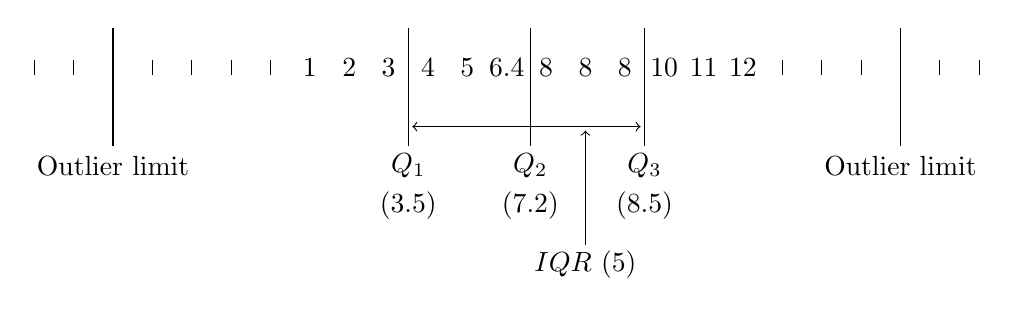
\begin{tikzpicture}

    % \node at (-5, 0) {-6};
    \draw[-] (-5, 0.1) -- (-5, -0.1);
    % \node at (-4.5, 0) {-5};
    \draw[-] (-4.5, 0.1) -- (-4.5, -0.1);
    % \node at (-4, 0) {-4};
    \draw[-] (-4, 0.1) -- (-4, -0.1);
    % \node at (-3.5, 0) {-3};
    \draw[-] (-3.5, 0.1) -- (-3.5, -0.1);
    % \node at (-3, 0) {-2};
    \draw[-] (-3, 0.1) -- (-3, -0.1);
    % \node at (-2.5, 0) {-1};
    \draw[-] (-2.5, 0.1) -- (-2.5, -0.1);
    % \node at (-2, 0) {0};
    \draw[-] (-2, 0.1) -- (-2, -0.1);
    \node at (-1.5, 0) {1};
    \node at (-1, 0) {2};
    \node at (-0.5, 0) {3};
    \node at (0, 0) {4};
    \node at (0.5, 0) {5};
    \node at (1, 0) {6.4};
    \node at (1.5, 0) {8};
    \node at (2, 0) {8};
    \node at (2.5, 0) {8};
    \node at (3, 0) {10};
    \node at (3.5, 0) {11};
    \node at (4, 0) {12};
    % \node at (4.5, 0) {13};
    \draw[-] (4.5, 0.1) -- (4.5, -0.1);
    % \node at (5, 0) {14};
    \draw[-] (5, 0.1) -- (5, -0.1);
    % \node at (5.5, 0) {15};
    \draw[-] (5.5, 0.1) -- (5.5, -0.1);
    % \node at (6, 0) {16};
    \draw[-] (6, 0.1) -- (6, -0.1);
    % \node at (6.5, 0) {17};
    \draw[-] (6.5, 0.1) -- (6.5, -0.1);
    % \node at (7, 0) {18};
    \draw[-] (7, 0.1) -- (7, -0.1);    

    \draw[-] (-0.25, 0.5) -- (-0.25, -1);
    \node at (-0.25, -1.25) {$Q_{1}$};
    \node at (-0.25, -1.75) {(3.5)};

    \draw[-] (1.3, 0.5) -- (1.3, -1);
    \node at (1.3, -1.25) {$Q_{2}$};
    \node at (1.3, -1.75) {(7.2)};

    \draw[-] (2.75, 0.5) -- (2.75, -1);
    \node at (2.75, -1.25) {$Q_{3}$};
    \node at (2.75, -1.75) {(8.5)}; 

    \draw[<->] (-0.2, -0.75) -- (2.7, -0.75);
    \draw[<-] (2, -0.8) -- (2, -2.25);
    \node at (2, -2.5) {$IQR$ (5)};

    \draw[-] (-4, 0.5) -- (-4, -1);
    \node at (-4, -1.25) {Outlier limit};

    \draw[-] (6, 0.5) -- (6, -1);
    \node at (6, -1.25) {Outlier limit};

  \end{tikzpicture}
\end{center}


\subsubsection{How to calculate it}

How far out are the outlier limits? The outlier limits are one and a half times the $IQR$ away from $Q_{1}$ or $Q_{3}$. So first calculate one and a half times the $IQR$:

\begin{equation*}
  1.5 * IQR
\end{equation*}

\noindent
In our example, the $IQR$ is 5, so we get 7.5:

\begin{equation*}
  1.5 * IQR = 1.5 * 5 = 7.5
\end{equation*}

\noindent
Then, to calculate the bottom outlier limit, \emph{subtract} that number from $Q_{1}$. This will tell us how low we can go below $Q_{1}$ before we hit the land of lower outliers:

\begin{equation*}
  \text{Lower outlier limit} = Q_{1} - (1.5 * IQR)
\end{equation*}

\noindent
In our example, the lower outlier limit is this:

\begin{equation*}
  \text{Lower outlier limit} = Q_{1} - (1.5 * IQR) = 3.5 - (1.5 * 5) = 3.5 - 7.5 = -4
\end{equation*}

\noindent
Any value that is smaller than that (that is to say, smaller than -4) is an outlier.

To compute the upper outlier limit, \emph{add} $1.5 * IQR$ to $Q_{3}$. This will tell us how high we can go above $Q_{3}$ before we hit the land of upper outliers:

\begin{equation*}
  \text{Upper outlier limit} = Q_{3} + (1.5 * IQR)
\end{equation*}

\noindent
In our example, the upper outlier limit is this:

\begin{equation*}
  \text{Upper outlier limit} = Q_{3} + (1.5 * IQR) = 8.5 + (1.5 * 5) = 8.5 + 7.5 = 16
\end{equation*}

\noindent
So any number in the data set bigger than that (that is to say, bigger than 16) is an outlier. Here is the picture, with the numbers marked on it:

\begin{center}
  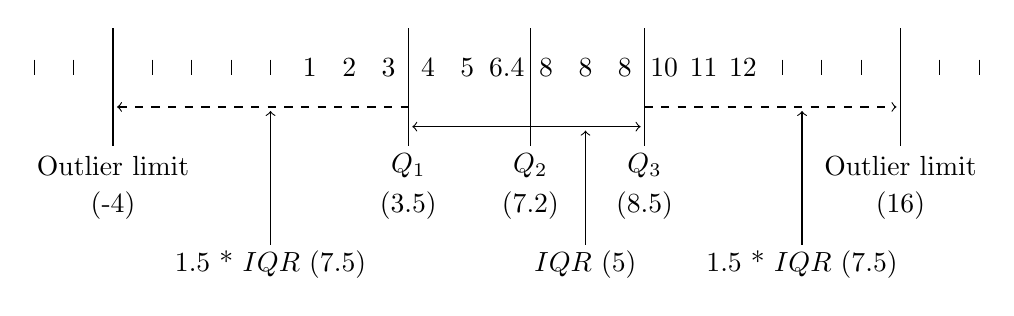
\begin{tikzpicture}

    % \node at (-5, 0) {-6};
    \draw[-] (-5, 0.1) -- (-5, -0.1);
    % \node at (-4.5, 0) {-5};
    \draw[-] (-4.5, 0.1) -- (-4.5, -0.1);
    % \node at (-4, 0) {-4};
    \draw[-] (-4, 0.1) -- (-4, -0.1);
    % \node at (-3.5, 0) {-3};
    \draw[-] (-3.5, 0.1) -- (-3.5, -0.1);
    % \node at (-3, 0) {-2};
    \draw[-] (-3, 0.1) -- (-3, -0.1);
    % \node at (-2.5, 0) {-1};
    \draw[-] (-2.5, 0.1) -- (-2.5, -0.1);
    % \node at (-2, 0) {0};
    \draw[-] (-2, 0.1) -- (-2, -0.1);
    \node at (-1.5, 0) {1};
    \node at (-1, 0) {2};
    \node at (-0.5, 0) {3};
    \node at (0, 0) {4};
    \node at (0.5, 0) {5};
    \node at (1, 0) {6.4};
    \node at (1.5, 0) {8};
    \node at (2, 0) {8};
    \node at (2.5, 0) {8};
    \node at (3, 0) {10};
    \node at (3.5, 0) {11};
    \node at (4, 0) {12};
    % \node at (4.5, 0) {13};
    \draw[-] (4.5, 0.1) -- (4.5, -0.1);
    % \node at (5, 0) {14};
    \draw[-] (5, 0.1) -- (5, -0.1);
    % \node at (5.5, 0) {15};
    \draw[-] (5.5, 0.1) -- (5.5, -0.1);
    % \node at (6, 0) {16};
    \draw[-] (6, 0.1) -- (6, -0.1);
    % \node at (6.5, 0) {17};
    \draw[-] (6.5, 0.1) -- (6.5, -0.1);
    % \node at (7, 0) {18};
    \draw[-] (7, 0.1) -- (7, -0.1);    

    \draw[-] (-0.25, 0.5) -- (-0.25, -1);
    \node at (-0.25, -1.25) {$Q_{1}$};
    \node at (-0.25, -1.75) {(3.5)};

    \draw[-] (1.3, 0.5) -- (1.3, -1);
    \node at (1.3, -1.25) {$Q_{2}$};
    \node at (1.3, -1.75) {(7.2)};

    \draw[-] (2.75, 0.5) -- (2.75, -1);
    \node at (2.75, -1.25) {$Q_{3}$};
    \node at (2.75, -1.75) {(8.5)}; 

    \draw[<->] (-0.2, -0.75) -- (2.7, -0.75);
    \draw[<-] (2, -0.8) -- (2, -2.25);
    \node at (2, -2.5) {$IQR$ (5)};

    \draw[-] (-4, 0.5) -- (-4, -1);
    \node at (-4, -1.25) {Outlier limit};
    \node at (-4, -1.75) {(-4)};

    \draw[<-,dashed] (-3.95, -0.5) -- (-0.25, -0.5);
    \draw[<-] (-2, -0.55) -- (-2, -2.25);
    \node at (-2, -2.5) {1.5 * $IQR$ (7.5)};

    \draw[-] (6, 0.5) -- (6, -1);
    \node at (6, -1.25) {Outlier limit};
    \node at (6, -1.75) {(16)};

    \draw[->,dashed] (2.75, -0.5) -- (5.95, -0.5);
    \draw[<-] (4.75, -0.55) -- (4.75, -2.25);
    \node at (4.75, -2.5) {1.5 * $IQR$ (7.5)};

  \end{tikzpicture}
\end{center}

\noindent
In this set of observations, all of the values are between 1 and 12, so there are no outliers. But if you encounter a set of observations that do have outliers, it is a good idea to consider those outliers, and figure out why exactly they are there. Sometimes outliers indicate mistakes in measurement or data collection, but sometimes they offer a key insight into your data.


%%%%%%%%%%%%%%%%%%%%%%%%%%%%%%%%%%%%%%%%%
\subsection{Interpreting quartiles}

Once we have cut up the data into quartiles, we can say which quartiles the values fall in. To use the current example:

\begin{itemize}
  \item What about 5? We say that 5 is \vocab{in the 2nd quartile}.
  \item What about 3? 3 is \vocab{in the 1st quartile}.
  \item What about 8? 8 is \vocab{in the 3rd quartile}.
  \item What about 11? 11 is \vocab{in the 4th quartile}.
\end{itemize}

\noindent
What do quartiles tell us? Each quartile tells us how many of the values in the data set have a value less than or equal to it. Because the values are ordered, go to any quartile, and you know that the values below it are going to be equal to or less than the quartile value. To use the current example again:

\begin{itemize}
  \item $Q_{1}$ is 3.5. This means that \vocab{25\% of the values} in the data set are \vocab{equal to or less than} 3.5. Look at the example above. One quarter of the values are indeed less than or equal to 3.5.
  \item $Q_{2}$ is 7.2. This means that \vocab{50\% of the values} in the data set are \vocab{equal to or less than} 7.2. Look at the example again. One half of the values are indeed less than or equal to 7.2.
  \item $Q_{3}$ is 8.5. This means that \vocab{75\% of the values} in the data set are \vocab{equal to or less than} 8.5. Confirm this in the example too.
\end{itemize}


%%%%%%%%%%%%%%%%%%%%%%%%%%%%%%%%%%%%%%%%%
%%%%%%%%%%%%%%%%%%%%%%%%%%%%%%%%%%%%%%%%%
\section{Percentiles}

Percentiles are just like the median and quartiles, except we divide the data up into 100 equal parts. We could manually divide up a data set, as we did above for the median and quartiles, but that would be very tedious to make 100 divisions. Fortunately, we can just think in terms of percentages, to figure out what we need to know.


%%%%%%%%%%%%%%%%%%%%%%%%%%%%%%%%%%%%%%%%%
\subsection{Calculating percentages}

Calculating percentiles is based on calculating percentages. How do we calculate the percentages? We use proportions. Percentages are basically just proportions, and proportions are just fractions. 50\% is one half, 75\% is three quarters, 23\% is $\frac{23}{100}$.


\subsubsection{Calculating the percentage}

Before going any further, let us stop to think about what percentages and proportions are, and how they are calculated. 

\begin{itemize}

  \item A \vocab{proportion} of a whole is some number taken out of the whole. For example, 3 out of 4, or 11 out of 257. This can be written as a fraction, because that is precisely what a fraction is! A fraction is precisely a \emph{fraction} of a whole. So, 3 out of 4 is $\frac{3}{4}$, and 11 out of 257 is $\frac{11}{257}$. We can also represent these as decimal values, by dividing the top number by the bottom number on a calculater. For example, $\frac{3}{4}$ is 0.75, and $\frac{11}{257}$ is 0.043.
  
  \item A \vocab{percentage} is just a proportion, put on a scale of 0 to 100. To put a proportion on a scale of 100, we simply multiply the proportion by 100. So the proportion 0.75, as a percentage, is 75\%, because 0.75 * 100 is 75. Similarly, the proportion 0.043, as a percentage, is 4.3\%, because 0.043 * 100 is 4.3.

\end{itemize}

\noindent
Suppose you have a collection of $n$ objects. Now take out $k$ of them. What proportion of the whole did we take out? We took $k$ out of $n$. As a fraction: $\frac{k}{n}$. If you want the decimal version of a fraction, simply divide $k$ by $n$ on a calculator. So here is the formula:

\begin{equation*}
  proportion = \frac{k}{n}
\end{equation*}

\noindent
For example, if we have a collection of 10 objects, and we take out 5 of them, then the proportion we remove is 5 out of 10, or $\frac{5}{10}$, which is really one half, or 0.5:

\begin{equation*}
  \frac{k}{n} = \frac{5}{10} = \frac{1}{2} = 0.5
\end{equation*}

\noindent
If we have a collection of 4 objects, and we take out 3 of them, the proportion we remove is 3 out of 4, or $\frac{3}{4}$ (0.75). 

\begin{equation*}
  \frac{k}{n} = \frac{3}{4} = 0.75
\end{equation*}

\noindent
If we have a collection of 14 objects, and we take out 8 of them, the proportion we remove is 8 out of 14, or $\frac{8}{14}$, i.e., 0.57.

\begin{equation*}
  \frac{k}{n} = \frac{8}{14} = \frac{4}{7} = 0.57
\end{equation*}

\noindent
To convert the decimal values into a percentage, multiply the proportion by 100. So, the percentage formula is this:

\begin{equation*}
  percentage = proportion * 100 = \frac{k}{n} * 100
\end{equation*}

\noindent
Hence, $\frac{5}{10}$ is 50\%:

\begin{equation*}
  \frac{k}{n} * 100 = \frac{5}{10} * 100 = 0.5 * 100 = 50
\end{equation*}

\noindent
And $\frac{3}{4}$ is 75\%:

\begin{equation*}
  \frac{k}{n} * 100 = \frac{3}{4} * 100 = 0.75 * 100 = 75
\end{equation*}

\noindent
And $\frac{8}{14}$ is 57\%:

\begin{equation*}
  \frac{k}{n} * 100 = \frac{8}{14} * 100 =  = \frac{4}{7} * 100 = 0.57 * 100 = 57
\end{equation*}

\noindent
To convert a percentage back into a proportion, divide by 100: 

\begin{equation*}
  proportion = \frac{percentage}{100}
\end{equation*}

\noindent
So, 50\% is .5, 75\% is 0.75, and 57\% is 0.57:

\begin{equation*}
  \frac{percentage}{100} = \frac{50}{100} = 0.5 \hskip 0.5cm 
  \frac{75}{100} = 0.75 \hskip 0.5cm
  \frac{57}{100} = 0.57
\end{equation*}



\subsubsection{Finding how many objects are in a proportion}

Suppose we have removed 75\% of the objects from a collection of 20 objects. How many objects have we removed? One way to figure it out is this. First, we know that 75\% is $\frac{3}{4}$. So we can divide the total collection up into 4 parts to find out how many objects are in one of the 4 parts:

\begin{equation*}
  \frac{20}{4} = 5
\end{equation*}

\noindent
Hence, there are 5 objects in each one of the four parts. But we want to know how big \emph{three} parts are, not just \emph{one} part. So, to calculate the total size of 3 of the parts added together, we need to add 5 to itself 3 times (which is the same as multiplying 5 by 3):

\begin{equation*}
  5 + 5 + 5 = 5 * 3 = 15
\end{equation*}

\noindent
Now we know that three of the four parts has 15 objects in it. Hence, if we remove three out of the four parts of a collection of 20, we remove 15 objects. That is to say, 75\% of 20 is 15.

Notice what we did. We divided the total by 4, and then we multiplied that by 3:

\begin{equation*}
  \frac{20}{4} * 3
\end{equation*}

\noindent
We can write this another way:

\begin{equation*}
  20 * \frac{1}{4} * 3 \hskip 1cm \text{which is really: } \hskip 1cm 20 * \frac{3}{4}
\end{equation*}

\noindent
In other words, we can multiply the total number (20) by the proportion ($\frac{3}{4}$), and that will tell us how big (how many objects) three-quarters of 20 is.

To make it even simpler, we can replace the fraction $\frac{3}{4}$ with its decimal value, i.e. 0.75 .Then the equation becomes:

\begin{equation*}
  20 * \frac{3}{4} = 20 * 0.75
\end{equation*}

\noindent
This shows us that, if you want to know how big 75\% of 20 is, we can convert the percentage into the decimal proportion (i.e., divide 75 by 100), and then multiply that by 20:

\begin{equation*}
  75\% = \frac{75}{100} = 0.75 \hskip 0.5cm \text{ and } \hskip 0.5cm 20 * 0.75 = 20 * 0.75
\end{equation*}

\noindent
Let's put that into a formula. To calculate how big $p$\% of $n$ objects are, do this:

\begin{equation*}
  n * \frac{p}{100}
\end{equation*}

\noindent
Here is another example. Suppose we have removed 50\% of a collection of 10 objects. How many objects have we removed? In this case, we know that we have removed 50\% of the total, which is one half. So, if we divide the total number of objects (10) by 2, we find out how big each half is:

\begin{equation*}
  \frac{10}{2} = 5
\end{equation*}

\noindent
Another way to do the same thing:

\begin{equation*}
  10 * \frac{1}{2} = 5
\end{equation*}

\noindent
Or, to use the formula:

\begin{equation*}
  n * \frac{p}{100} = 10 * \frac{50}{100} = 10 * 0.5 = 5
\end{equation*}



%%%%%%%%%%%%%%%%%%%%%%%%%%%%%%%%%%%%%%%%%
\subsection{The percentage of values below a number}

Suppose you pick a number in a data set, and you want to find out what percentage of the values in the whole data set are smaller than the number you picked. Let's call the number you picked $k$. In statistics, we say that here you want to find \vocab{the percentile \emph{of} $k$}.

For example, suppose we roll a six sided dice 8 times, and we roll these numbers:

\begin{equation*}
  5, 1, 6, 1, 4, 2, 4, 3
\end{equation*}

\noindent
Now pick a number in this data set, for example 5. What percentage of all the observations are smaller than 5? 


\subsubsection{Rough approximation}

To get a rough approximation, first order the observations from smallest to largest:

\begin{equation*}
  1, 1, 2, 3, 4, 4, 5, 6
\end{equation*}

\noindent
Next, count how many observations there are in the whole data set. In this case, there are 8 observations (because we rolled the dice 8 times).

Now, count how many observations have a value less than or equal to 5. In this case, there are 7 observation that have a value of 5 or less.

Think about what we know now. We know that 7 out of the 8 total observations have a value of 5 or less. And 7 out of 8 is a fraction: $\frac{7}{8}$ of the observations have a value of 5 or less. 

To convert that to a percentage, simply divide 7 by 8, which gives us 0.875, or 87.5\%. And that is our answer: 87.5\% of the observations have a value of 5 or less.


\subsubsection{A slightly better approximation}

Suppose we want to know what percentage of the observations have a value of 4 or less. In our data set, there are 6 observations that have a value of 4 or less. And 6 out of 8 is 0.75 (6 / 8 = 0.75), or 75\%. So we could say that 75\% of the observations have a value of 4 or less.

If we like, we can weight each of the 4s a little less. To do that, we can count each 4 as only half of an observation. There are 2 observations that have a value of 4, and if each one only counts as half an observation, together they add up to 1 observation (0.5 observation + 0.5 observation = 1 observation).

You can compute this by counting how many observations have the value in question --- let us call this $y$ --- and then multiply that number of 0.5:

\begin{equation*}
  0.5 * y 
\end{equation*}

\noindent
or just:

\begin{equation*}
  0.5y
\end{equation*}

In our example, $y$ is 2, so:

\begin{equation*}
  0.5 * 2 = 1
\end{equation*}

\noindent
Beyond that, there are 4 other observations that have a value less than 4. These are the observations with values of 1, 1, 2, and 3. Each of these observations counts as a full observation. Let us call this number $x$.

To get all the observations, we add up $x$ (the full observations), plus $y * 0.5$ (the half observations). Hence:

\begin{equation*}
  x + 0.5y
\end{equation*}

\noindent
Then we divide that number by the total number of observations $n$:

\begin{equation*}
  \frac{x + 0.5y}{n}
\end{equation*}

\noindent
In our case, we have 4 full observations, and 2 half observations, so we have 5 observations with a value of 4 or less, out of the total 8 observations:

\begin{equation*}
  \frac{x + 0.5y}{n} = \frac{4 + (0.5 * 2)}{8} = \frac{5}{8} = 0.625
\end{equation*}

\noindent
To get a percentage, we multiply that by 100, so the full formula is:

\begin{equation*}
  \frac{x + 0.5y}{n} * 100 = \frac{4 + (0.5 * 2)}{8} * 100 = \frac{5}{8} * 100 = 0.625 * 100 = 62.5
\end{equation*}

\noindent
So 62.5\% of the observations have a value of 4 or less, using this slightly better approximation.


%%%%%%%%%%%%%%%%%%%%%%%%%%%%%%%%%%%%%%%%%
\subsection{The $k$th percentile}

Suppose we take a data set and order the observations from the smallest to largest values. Suppose next that we want to take 75\% of the values, and we want to know the top value in those observations. In statistics, we say that here you want to find \vocab{the $k$th percentile}.

For example, suppose we have 8 observations which have been arranged from lowest to highest. For the moment, let's ignore what the values actually are. Let's just think of them as boxes that have values inside.

\begin{center}
  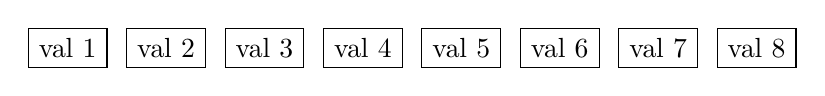
\begin{tikzpicture}

    \node at (-5, 0) {val 1};
    \draw[-] (-5.5, -0.25) -- (-4.5, -0.25) -- (-4.5, 0.25) -- (-5.5, 0.25) -- (-5.5, -0.25);

    \node at (-3.75, 0) {val 2};
    \draw[-] (-4.25, -0.25) -- (-3.25, -0.25) -- (-3.25, 0.25) -- (-4.25, 0.25) -- (-4.25, -0.25);

    \node at (-2.5, 0) {val 3};
    \draw[-] (-3, -0.25) -- (-2, -0.25) -- (-2, 0.25) -- (-3, 0.25) -- (-3, -0.25);

    \node at (-1.25, 0) {val 4};
    \draw[-] (-1.75, -0.25) -- (-0.75, -0.25) -- (-0.75, 0.25) -- (-1.75, 0.25) -- (-1.75, -0.25);

    \node at (0, 0) {val 5};
    \draw[-] (-0.5, -0.25) -- (0.5, -0.25) -- (0.5, 0.25) -- (-0.5, 0.25) -- (-0.5, -0.25);

    \node at (1.25, 0) {val 6};
    \draw[-] (1.75, -0.25) -- (0.75, -0.25) -- (0.75, 0.25) -- (1.75, 0.25) -- (1.75, -0.25);

    \node at (2.5, 0) {val 7};
    \draw[-] (3, -0.25) -- (2, -0.25) -- (2, 0.25) -- (3, 0.25) -- (3, -0.25);

    \node at (3.75, 0) {val 8};
    \draw[-] (4.25, -0.25) -- (3.25, -0.25) -- (3.25, 0.25) -- (4.25, 0.25) -- (4.25, -0.25);

  \end{tikzpicture}
\end{center}

\noindent
Now we want to take 75\% of those observations:

\begin{center}
  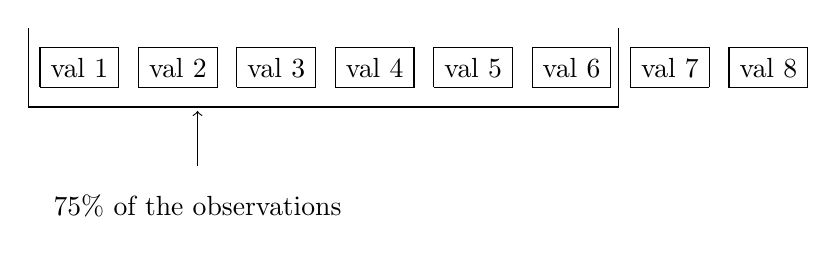
\begin{tikzpicture}

    \node at (-5, 0) {val 1};
    \draw[-] (-5.5, -0.25) -- (-4.5, -0.25) -- (-4.5, 0.25) -- (-5.5, 0.25) -- (-5.5, -0.25);

    \node at (-3.75, 0) {val 2};
    \draw[-] (-4.25, -0.25) -- (-3.25, -0.25) -- (-3.25, 0.25) -- (-4.25, 0.25) -- (-4.25, -0.25);

    \node at (-2.5, 0) {val 3};
    \draw[-] (-3, -0.25) -- (-2, -0.25) -- (-2, 0.25) -- (-3, 0.25) -- (-3, -0.25);

    \node at (-1.25, 0) {val 4};
    \draw[-] (-1.75, -0.25) -- (-0.75, -0.25) -- (-0.75, 0.25) -- (-1.75, 0.25) -- (-1.75, -0.25);

    \node at (0, 0) {val 5};
    \draw[-] (-0.5, -0.25) -- (0.5, -0.25) -- (0.5, 0.25) -- (-0.5, 0.25) -- (-0.5, -0.25);

    \node at (1.25, 0) {val 6};
    \draw[-] (1.75, -0.25) -- (0.75, -0.25) -- (0.75, 0.25) -- (1.75, 0.25) -- (1.75, -0.25);

    \node at (2.5, 0) {val 7};
    \draw[-] (3, -0.25) -- (2, -0.25) -- (2, 0.25) -- (3, 0.25) -- (3, -0.25);

    \node at (3.75, 0) {val 8};
    \draw[-] (4.25, -0.25) -- (3.25, -0.25) -- (3.25, 0.25) -- (4.25, 0.25) -- (4.25, -0.25);

    \draw[-] (-5.65, 0.5) -- (-5.65, -0.5) -- (1.85, -0.5) -- (1.85, 0.5);
    \draw[<-] (-3.5, -0.55) -- (-3.5, -1.25);
    \node at (-3.5, -1.75) {75\% of the observations};

  \end{tikzpicture}
\end{center}

\noindent
And we want to get the value in the very top box:

\begin{center}
  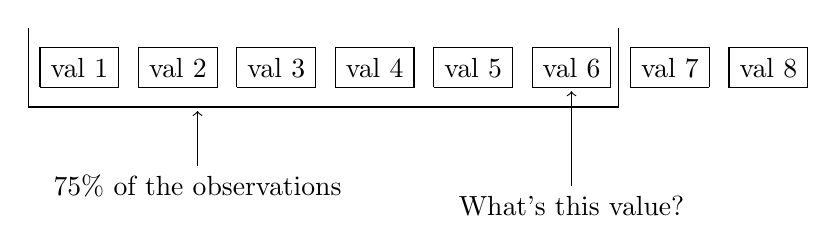
\begin{tikzpicture}

    \node at (-5, 0) {val 1};
    \draw[-] (-5.5, -0.25) -- (-4.5, -0.25) -- (-4.5, 0.25) -- (-5.5, 0.25) -- (-5.5, -0.25);

    \node at (-3.75, 0) {val 2};
    \draw[-] (-4.25, -0.25) -- (-3.25, -0.25) -- (-3.25, 0.25) -- (-4.25, 0.25) -- (-4.25, -0.25);

    \node at (-2.5, 0) {val 3};
    \draw[-] (-3, -0.25) -- (-2, -0.25) -- (-2, 0.25) -- (-3, 0.25) -- (-3, -0.25);

    \node at (-1.25, 0) {val 4};
    \draw[-] (-1.75, -0.25) -- (-0.75, -0.25) -- (-0.75, 0.25) -- (-1.75, 0.25) -- (-1.75, -0.25);

    \node at (0, 0) {val 5};
    \draw[-] (-0.5, -0.25) -- (0.5, -0.25) -- (0.5, 0.25) -- (-0.5, 0.25) -- (-0.5, -0.25);

    \node at (1.25, 0) {val 6};
    \draw[-] (1.75, -0.25) -- (0.75, -0.25) -- (0.75, 0.25) -- (1.75, 0.25) -- (1.75, -0.25);

    \node at (2.5, 0) {val 7};
    \draw[-] (3, -0.25) -- (2, -0.25) -- (2, 0.25) -- (3, 0.25) -- (3, -0.25);

    \node at (3.75, 0) {val 8};
    \draw[-] (4.25, -0.25) -- (3.25, -0.25) -- (3.25, 0.25) -- (4.25, 0.25) -- (4.25, -0.25);

    \draw[-] (-5.65, 0.5) -- (-5.65, -0.5) -- (1.85, -0.5) -- (1.85, 0.5);
    \draw[<-] (-3.5, -0.55) -- (-3.5, -1.25);
    \node at (-3.5, -1.5) {75\% of the observations};
    
    \draw[<-] (1.25, -0.30) -- (1.25, -1.5);
    \node at (1.25, -1.75) {What's this value?};

  \end{tikzpicture}
\end{center}

\noindent
That value is what we call the \vocab{75th percentile}. We call it that, because it is the value that 75\% of the observations are smaller than or equal to. That value divides the bottom 75\% of the observations off from the top 25\% of the observations.

The same goes for any other $k$th percentile. For example, the 50th percentile is the value that 50\% of the observations are smaller than or equal to. Similarly, the 28th percentile is the value that 28\% of the observations are smaller than or equal to.


\subsubsection{Rough approximation}

To find the $k$th percentile, what we have to find is which box has the value we want. To find the right box, we need to know how many boxes we should count to, starting from the left. In the above example, we need to count 6 boxes over from the left, and that gets us the box we want. Then we open up that box and look inside, and there we have our value.

How do we figure out how many boxes to count over? Well, if we want the 75th percentile, we need to count over 75\% of the total boxes. If we want the 50\% percentile, we need to count over 50\% of the total boxes. If we want the $k$th percentile, we need to count over $k$\% of the total boxes.

How do we find $k$ percent of the total boxes? Multiply $\frac{k}{100}$ by the total number of boxes $n$:

\begin{equation*}
  \frac{k}{100} * n
\end{equation*}

\noindent
For example, 75\% of 8 boxes is 6:

\begin{equation*}
  \frac{75}{100} * 8 = 0.75 * 8 = 6
\end{equation*}

\noindent
So, we count over 6 boxes. Then we look in that box, and that is our 75th percentile value. Similarly, 50\% of 8 boxes is 4:

\begin{equation*}
  \frac{50}{100} * 8 = 0.5 * 8 = 4
\end{equation*}

\noindent
So we count over 4 boxes, and the value in that box is our 50th percentile value. Likewise, 35\% of 8 boxes is 2.8:

\begin{equation*}
  \frac{35}{100} * 8 = 0.35 * 8 = 2.8
\end{equation*}

\noindent
So, we count over about 2.8 boxes, i.e., 3 boxes (after we round it up), and the value we find in that box is our 35th percentile value.


\subsubsection{A slightly better approximation}

In the last example, we needed to round up to get to the closest box. We really want to round \emph{up} here, to ensure that we select a value that is \emph{bigger} than the other $k$\% of the values. By rounding up, we always end up with a value that $k$ percent of the observations are \emph{smaller than} or equal to.

To make this happen, we can just add one to $n$ when we do the calculation. So the equation becomes this:

\begin{equation*}
  \frac{k}{100} * (n + 1)
\end{equation*}

\noindent
If the result is a whole number, then that is our $k$th percentile. If the result is a fraction between two numbers $m$ and $n$, we can just say the $k$th percentile is the midway point between $m$ and $n$. To find that, we add the two numbers $m$ and $n$ and divide by two. For example, if we end up with the $k$th percentile being 4.67, between 4 and 5.5, we can add 4 to 5.5, and divide by 2:

\begin{equation*}
  \frac{4 + 5.5}{2} = \frac{9.5}{2} = 4.75
\end{equation*}

\noindent
Similarly, if the result is 5.6, between 5 and 7, we can add 5 to 7, and divide by 2:

\begin{equation*}
  \frac{5 + 7}{2} = \frac{12}{2} = 6
\end{equation*}


\end{document}
